\let\negmedspace\undefined
\let\negthickspace\undefined
\documentclass[journal,12pt,onecolumn]{IEEEtran}
\usepackage{cite}
\usepackage{amsmath,amssymb,amsfonts,amsthm}
\usepackage{algorithmic}
\usepackage[version=4]{mhchem}
\usepackage{graphicx}
\usepackage{textcomp}
\usepackage{xcolor}
\usepackage{amsmath}
\usepackage{txfonts}
\usepackage{listings}
\usepackage{enumitem}
\usepackage{mathtools}
\usepackage{gensymb}
\usepackage{comment}
\usepackage[breaklinks=true]{hyperref}
\usepackage{tkz-euclide} 
\usepackage{gvv}                                        
%\def\inputGnumericTable{}                                 
\usepackage[latin1]{inputenc}     
\usepackage{xparse}
\usepackage{color}
\usepackage{array}                                         
\usepackage{longtable}                                     
\usepackage{calc}                                          
\usepackage{multirow}
\usepackage{multicol}
\usepackage{hhline}                                        
\usepackage{ifthen}                                        
\usepackage{lscape}
\usepackage{tabularx}
\usepackage{array}
\usepackage{float}
\newtheorem{theorem}{Theorem}[section]
\newtheorem{problem}{Problem}
\newtheorem{proposition}{Proposition}[section]
\newtheorem{lemma}{Lemma}[section]
\newtheorem{corollary}[theorem]{Corollary}
\newtheorem{example}{Example}[section]
\newtheorem{definition}[problem]{Definition}
\newcommand{\BEQA}{\begin{eqnarray}}
\newcommand{\EEQA}{\end{eqnarray}}
\newcommand{\define}{\stackrel{\triangle}{=}}
\theoremstyle{remark}
\newtheorem{rem}{Remark}
% Marks the beginning of the document
\begin{document}
\title{gg Gate 2015}
\author{ai25btech11014-Gooty Suhas}
\maketitle
\section*{General Aptitude (GA) Questions}

\begin{enumerate}
\item Choose the appropriate word/phrase, out of the four options given below, to complete the following sentence:  
Apparent lifelessness \underline{\hspace{1cm}} dormant life.  
\begin{multicols}{4}
\begin{enumerate}
\item harbours  
\item leads to  
\item supports  
\item affects  
\end{enumerate}
\end{multicols}

\item Fill in the blank with the correct idiom/phrase.  
That boy from the town was a \underline{\hspace{1cm}} in the sleepy village.  
\begin{multicols}{2}
\begin{enumerate}
\item dog out of herd  
\item sheep from the heap  
\item fish out of water  
\item bird from the flock  
\end{enumerate}
\end{multicols}

\item Choose the statement where the underlined word is used correctly.  
\begin{enumerate}
\item When the teacher eludes to different authors, he is being elusive.  
\item When the thief keeps eluding the police, he is being elusive.  
\item Matters that are difficult to understand, identify or remember are allusive.  
\item Mirages can be allusive, but a better way to express them is illusory.  
\end{enumerate}

\item Tanya is older than Eric. Cliff is older than Tanya. Eric is older than Cliff.  
If the first two statements are true, then the third statement is:  
\begin{enumerate}
\item True  
\item False  
\item Uncertain  
\item Data insufficient  
\end{enumerate}

\item Five teams have to compete in a league, with every team playing every other team exactly once, before going to the next round.  
How many matches will have to be held to complete the league round of matches?  
\begin{multicols}{4}
\begin{enumerate}
\item 20  
\item 10  
\item 8  
\item 5  
\end{enumerate}
\end{multicols}

\item Select the appropriate option in place of the underlined part of the sentence.  
Increased productivity necessary reflects greater efforts made by the employees.  
\begin{enumerate}
\item Increase in productivity necessary  
\item Increase productivity is necessary  
\item Increase in productivity necessarily  
\item No improvement required  
\end{enumerate}

\item Given below are two statements followed by two conclusions. Assuming these statements to be true, decide which one logically follows.  
\textbf{Statements:}  
I. No manager is a leader.  
II. All leaders are executives.  

\textbf{Conclusions:}  
I. No manager is an executive.  
II. No executive is a manager.  
\begin{enumerate}
\item Only conclusion I follows.  
\item Only conclusion II follows.  
\item Neither conclusion I nor II follows.  
\item Both conclusions I and II follow.  
\end{enumerate}

\item In the given figure angle Q is a right angle, PS:QS = 3:1, RT:QT = 5:2 and PU:UR = 1:1.  
If area of triangle QTS is 20 cm\(^2\), then the area of triangle PQR in cm\(^2\) is  

\begin{figure}[H]
    \centering
    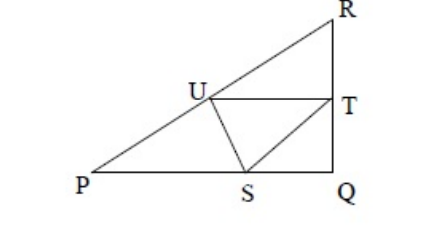
\includegraphics[width=0.3\textwidth]{figs/fig1.png}
    \caption{Image for questions 8}
    \label{fig:question8}
\end{figure}

\begin{multicols}{4}
\begin{enumerate}
\item 280  
\item 140  
\item 70  
\item 35  
\end{enumerate}
\end{multicols}

\item Right triangle PQR is to be constructed in the xy-plane so that the right angle is at P and line PR is parallel to the x-axis.  
The x and y coordinates of P, Q, and R are to be integers that satisfy the inequalities: \(-4 \leq x \leq 5\) and \(6 \leq y \leq 16\).  
How many different triangles could be constructed with these properties?  
\begin{multicols}{2}
\begin{enumerate}
\item 110  
\item 1,100  
\item 9,900  
\item 10,000  
\end{enumerate}
\end{multicols}

\item A coin is tossed thrice. Let X be the event that head occurs in each of the first two tosses.  
Let Y be the event that a tail occurs on the third toss.  
Let Z be the event that two tails occur in three tosses.  
Based on the above information, which one of the following statements is TRUE?  
\begin{multicols}{2}
\begin{enumerate}
\item X and Y are not independent  
\item Y and Z are dependent  
\item Y and Z are independent  
\item X and Z are independent  
\end{enumerate}
\end{multicols}

\end{enumerate}

\section*{Part A: Geology and Geophysics }
\vspace{0.5cm}

\begin{enumerate}
\setcounter{enumi}{10}

\item The shape of the earth is best described as  
\begin{multicols}{2}
\begin{enumerate}
\item spheroid  
\item prolate ellipsoid  
\item ellipsoid  
\item oblate spheroid  
\end{enumerate}
\end{multicols}

\item Which one amongst the following is the CORRECT attitude of a bed?  
\begin{multicols}{4}
\begin{enumerate}
\item 221°, 95°  
\item N45°W, 40°SE  
\item 090°/ 20°W  
\item 089°, 75°S  
\end{enumerate}
\end{multicols}

\item Hawaiian Island chain is the result of  
\begin{enumerate}
\item collision of two oceanic plates  
\item intraplate hot spot activity  
\item divergence of two oceanic plates  
\item interplate hot spot activity  
\end{enumerate}

\item In which one of the following configurations the electrodes are uniformly spaced?  
\begin{enumerate}
\item Schlumberger array  
\item Pole-dipole array  
\item Wenner array  
\item Pole-pole array  
\end{enumerate}

\item In Triclinic crystal system, the three crystallographic axes \(a, b, c\) are of  
\begin{enumerate}
\item equal lengths with angle between \(b\) and \(c\) as 90°  

\item equal lengths with angle between \( a \) and \( c \) such that \( \angle ac \neq 90^\circ \)  
\item unequal lengths with angle between \( a \) and \( c \) such that \( \angle ac \neq 90^\circ \)
\item unequal lengths with angle between \(b\) and \(c\) as 90°  
\end{enumerate}

\item A landform that results from free fall of rocks is called  
\begin{multicols}{4}
\begin{enumerate}
\item talus slope  
\item eskers  
\item alluvial fan  
\item debris flow  
\end{enumerate}
\end{multicols}

\item Which one of the following figures correctly depicts the geomagnetic declination (D) and inclination (I) angles?  
\begin{multicols}{2}
\begin{enumerate}
\item \begin{figure}[H]
    \centering
    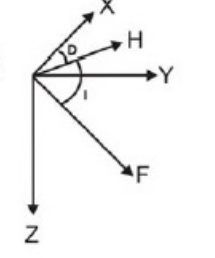
\includegraphics[width=0.1\textwidth]{figs/fig2.png}
    \caption{Image for questions 17}
    \label{fig:question17a}
\end{figure}

\item \begin{figure}[H]
    \centering
    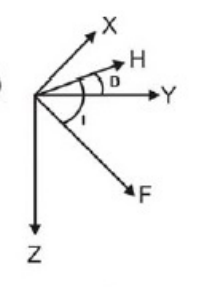
\includegraphics[width=0.1\textwidth]{figs/fig3.png}
    \caption{Image for questions 17}
    \label{fig:question17b}
\end{figure}

\item \begin{figure}[H]
    \centering
    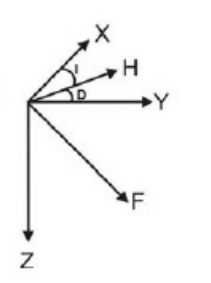
\includegraphics[width=0.1\textwidth]{figs/fig4.png}
    \caption{Image for questions 17}
    \label{fig:question17c}
\end{figure}

\item \begin{figure}[H]
    \centering
    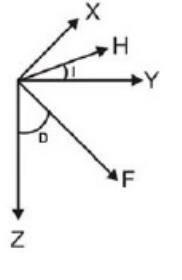
\includegraphics[width=0.1\textwidth]{figs/fig5.png}
    \caption{Image for questions 17}
    \label{fig:question17d}
\end{figure}

\end{enumerate}
\end{multicols}

\item Which one of the following logging methods is NOT used to determine porosity?  
\begin{multicols}{4}
\begin{enumerate}
\item Sonic  
\item SP  
\item Neutron  
\item Gamma-gamma  
\end{enumerate}
\end{multicols}

\item PcP and ScS phases are reflected from  
\begin{enumerate}
\item crust - mantle boundary  
\item core - mantle boundary  
\item inner core - outer core boundary  
\item lithosphere - asthenosphere boundary  
\end{enumerate}

\item Identify the CORRECT sequence of the electromagnetic waves in their increasing frequency  
\begin{enumerate}
\item radio wave, micro-wave, infrared, visible, ultra violet, X-ray  
\item radio wave, infrared, micro-wave, visible, ultra violet, X-ray  
\item micro-wave, radio wave, infrared, visible, X-ray, ultra violet  
\item infrared, visible, micro-wave, radio wave, X-ray, ultra violet  
\end{enumerate}

\item \textbf{(NAT)} Considering the Airy isostatic compensation for a mountain having elevation of 2.0 km above mean sea level at a point \(P\), the thickness of its root below \(P\) would be \underline{\hspace{3cm}} km.  
\vspace{0.5cm}

\item \textbf{(NAT)} The reflection coefficient at the interface separating sandstone (\(V_p = 2000\) m/s, \(\rho = 1.5\) g/cm\(^3\)) underlain by shale (\(V_p = 2500\) m/s, \(\rho = 2.0\) g/cm\(^3\)) is \underline{\hspace{3cm}}.  
\vspace{0.5cm}

\item Gardner's formula relates the seismic P-wave velocity (\(V_p\)) to  
\begin{multicols}{2}
\begin{enumerate}
\item density  
\item porosity  
\item permeability  
\item lithology  
\end{enumerate}
\end{multicols}

\item Which one of the following sedimentary basins is related to extension?  
\begin{multicols}{2}
\begin{enumerate}
\item foredeep  
\item half-graben  
\item piggyback  
\item fore-arc  
\end{enumerate}
\end{multicols}

\item In a seismic section, paraconformity is marked by  
\begin{multicols}{2}
\begin{enumerate}
\item onlap  
\item downlap  
\item erosional truncation  
\item concordance  
\end{enumerate}
\end{multicols}

\end{enumerate}

\begin{enumerate}
\setcounter{enumi}{25}

\item Match the names listed in Group I with the attributes listed in Group II.

\begin{multicols}{2}
\textbf{Group I}  
\begin{flushleft}
P. Carlsberg Ridge\\
Q. Ninetyeast Ridge\\
R. Pranhita-Godavari Basin\\
S. Makran Coast
\end{flushleft}

\columnbreak

\textbf{Group II}  
\begin{flushleft}
1. Aseismic\\
2. Subduction\\
3. Spreading\\
4. Transform\\
5. Rift
\end{flushleft}
\end{multicols}

\begin{multicols}{2}
\begin{enumerate}
\item P--5; Q--3; R--1; S--4  
\item P--3; Q--1; R--5; S--2  
\item P--3; Q--4; R--1; S--2  
\item P--1; Q--3; R--5; S--4  
\end{enumerate}
\end{multicols}

\item In India, bituminous coal occurs at  
\begin{multicols}{4}
\begin{enumerate}
\item Panandhro  
\item Palana  
\item Neyveli  
\item Jharia  
\end{enumerate}
\end{multicols}

\item On the Earth, all conditions being same, the time period of a simple pendulum will be maximum at the  
\begin{multicols}{2}
\begin{enumerate}
\item Poles  
\item Tropic of Cancer  
\item Tropic of Capricorn  
\item Equator  
\end{enumerate}
\end{multicols}

\item The two most abundant elements in the Earth are  
\begin{multicols}{2}
\begin{enumerate}
\item oxygen and iron  
\item iron and magnesium  
\item oxygen and silicon  
\item iron and silicon  
\end{enumerate}
\end{multicols}

\item The pair of curves that depicts the radioactive decay and growth of a parent-daughter pair is  

\begin{figure}[H]
    \centering
    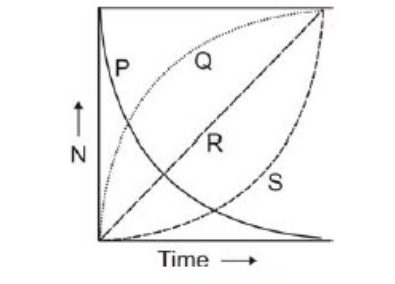
\includegraphics[width=0.4\textwidth]{figs/fig6.png}
    \caption{Image for questions 30}
    \label{fig:question30}
\end{figure}

\begin{multicols}{2}
\begin{enumerate}
\item P, Q  
\item P, R  
\item P, S  
\item S, Q  
\end{enumerate}
\end{multicols}

\item \textbf{(NAT)} A drainage basin with an area of \(2.0 \times 10^6\) m\(^2\) receives continuous rainfall for 48 hours at a uniform rate of 3 mm/h. The volume of precipitation is \underline{\hspace{3cm}} m\(^3\) of water.  
\vspace{0.6cm}

\item The main source of error in computing the orientation of planar features from drill cores is  
\begin{enumerate}
\item rotation of the core during extraction  
\item cylindrical shape of the core  
\item non-vertical orientation of the drill axis  
\item staining during drilling operations  
\end{enumerate}

\item Which combination of sorting and roundness of sand grains results in highest permeability?  
\begin{enumerate}
\item well sorted, poorly rounded  
\item well sorted, well rounded  
\item poorly sorted, poorly rounded  
\item poorly sorted, well rounded  
\end{enumerate}

\item Amongst the different gases in the atmosphere, which one of the following pairs DOES NOT contribute to heating of the atmosphere?  
\begin{multicols}{4}
\begin{enumerate}
\item CO\(_2\), H\(_2\)O  
\item N\(_2\), O\(_2\)  
\item H\(_2\)O, CH\(_4\)  
\item H\(_2\)O, O\(_3\)  
\end{enumerate}
\end{multicols}

\item The data of which one of the following active electromagnetic techniques can be used to correct static shift effect in magnetotelluric apparent resistivity data?  
\begin{multicols}{4}
\begin{enumerate}
\item Slingram  
\item Turam  
\item VLF  
\item TEM  
\end{enumerate}
\end{multicols}

\end{enumerate}


\begin{enumerate}
\setcounter{enumi}{35}

\item Which one of the following statements describing aspects of partial melting behavior of a binary eutectic system is NOT TRUE?  
\begin{enumerate}
\item Melting is complete at temperature just above the liquidus temperature.  
\item Two solid phases and one liquid phase co-exist at eutectic temperature.  
\item The lowest temperature at which partial melting occurs is independent of the chemical composition.  
\item The composition of the first liquid to form depends on the composition of the sample.  
\end{enumerate}

\item Find the CORRECT statement amongst the following.  
\begin{enumerate}
\item Delthyrium is a triangular cavity in cephalopod  
\item Madreporite is a skeletal part of Brachiopoda  
\item Pleuron is a part of thorax in Trilobite  
\item Endocone is the jaw of an Ammonoid  
\end{enumerate}

\item Which one of the following statements is NOT true regarding REEs partitioning?  

\begin{figure}[H]
    \centering
    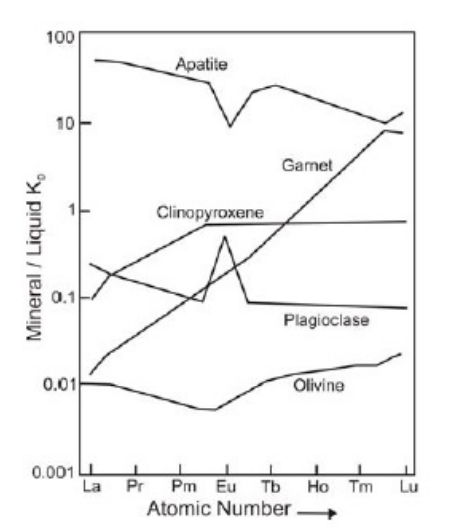
\includegraphics[width=0.4\textwidth]{figs/fig7.png}
    \caption{Image for questions 38}
    \label{fig:question38}
\end{figure}

\begin{enumerate}
\item REEs are compatible only in apatite.  
\item Heavy REEs are compatible whereas Light REEs are incompatible in garnet.  
\item REEs are incompatible only in apatite.  
\item REEs are incompatible in olivine.  
\end{enumerate}

\item Which one of the following is NOT a set of polymorphous minerals?  
\begin{enumerate}
\item calcite, aragonite, vaterite  
\item quartz, coesite, tridymite  
\item graphite, anthracite, diamond  
\item kyanite, sillimanite, andalusite  
\end{enumerate}

\item Chemical analysis reveals that basalts contain much more aluminum (Al\(_2\)O\(_3\) ~15%) in comparison to peridotites (Al\(_2\)O\(_3\) ~4%). This is because they contain  
\begin{enumerate}
\item very little olivine  
\item higher proportion of pyroxene  
\item feldspars as dominant mineral  
\item no quartz  
\end{enumerate}

\item \textbf{(NAT)} A sandstone bed whose attitude is $090^\circ$, $30^\circ$ is exposed on a flat surface. The true thickness of the bed is 100 m. The width of the outcrop of the sandstone bed along a N--S traverse on the ground is \underline{\hspace{3cm}} m.
\vspace{0.3cm}

\item Assertion (a): The \(^{18}\)O/\(^{16}\)O ratio in natural systems can be used as a thermometer.  
Reason (r): The fractionation of \(^{18}\)O/\(^{16}\)O depends on temperature.  
\begin{enumerate}
\item Both (a) and (r) are True and (r) is the correct reason for (a).  
\item Both (a) and (r) are not True.  
\item (a) is True but (r) is not True  
\item Both (a) and (r) are True but (r) is not the correct reason for (a).  
\end{enumerate}

\item Match the boreholes in Group I with their features in Group II.

\begin{figure}[H]
    \centering
    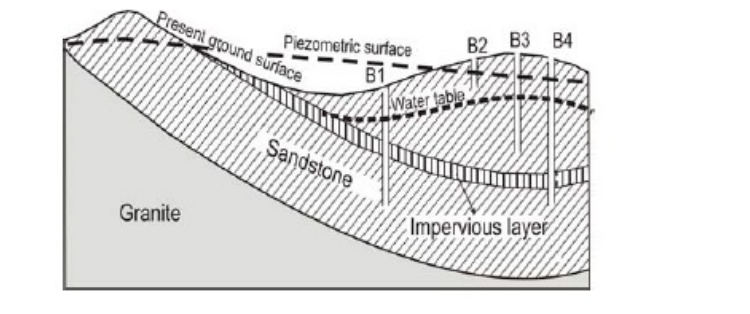
\includegraphics[width=0.6\textwidth]{figs/fig8.png}
    \caption{Image for questions 43}
    \label{fig:question43}
\end{figure}

\begin{multicols}{2}
\textbf{Group I}  
\begin{flushleft}
P. Borehole B1\\
Q. Borehole B2\\
R. Borehole B3\\
S. Borehole B4
\end{flushleft}

\columnbreak

\textbf{Group II}  
\begin{flushleft}
1. Well in unconfined aquifer\\
2. Artesian well with water not flowing to surface\\
3. Artesian well with water flowing to surface\\
4. Dry well
\end{flushleft}
\end{multicols}

\begin{multicols}{2}
\begin{enumerate}
\item P--1; Q--3; R--2; S--4  
\item P--2; Q--4; R--1; S--3  
\item P--3; Q--4; R--1; S--2  
\item P--3; Q--1; R--4; S--2  
\end{enumerate}
\end{multicols}

\item \textbf{(NAT)} If the total volume of water in the Earth's atmosphere is \(1.29 \times 10^4\) km\(^3\), and it were to uniformly cover the Earth's surface (area = \(5.1 \times 10^8\) km\(^2\)), the height of the resulting water column would be \underline{\hspace{3cm}} cm.  
\vspace{0.3cm}

\item \textbf{(NAT)} Samples of copper ores are drawn from locations X1, X2 and X3. The values of \%Cu at sampling locations are:  
X1 = 2.2\%, X2 = 1.1\%, X3 = 3.3\%.  
Using inverse distance weighting, the estimated grade at point X is \underline{\hspace{3cm}} \%.  

\begin{figure}[H]
    \centering
    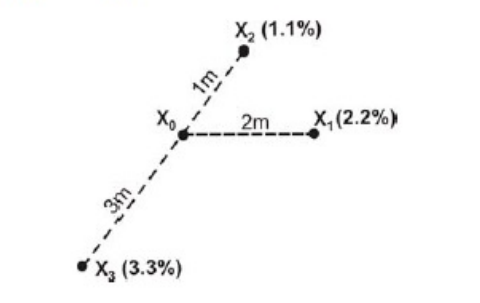
\includegraphics[width=0.4\textwidth]{figs/fig9.png}
    \caption{Image for questions 45}
    \label{fig:question45}
\end{figure}


\vspace{0.3cm}

\end{enumerate}

\begin{enumerate}
\setcounter{enumi}{45}

\item Match the point group (HM symbol) in Group I with its corresponding general form in Group II.

\begin{multicols}{2}
\textbf{Group I}  
\begin{flushleft}
P. 62m\\
Q. 3/m\\
R. 422\\
S. 42m
\end{flushleft}

\columnbreak

\textbf{Group II}  
\begin{flushleft}
1. Ditrigonal Dipyramid\\
2. Tetragonal Scalenohedron\\
3. Trigonal Dipyramid\\
4. Tetragonal Trapezohedron\\
5. Hexagonal Dipyramid
\end{flushleft}
\end{multicols}

\begin{multicols}{2}
\begin{enumerate}
\item P--5; Q--1; R--2; S--4  
\item P--1; Q--3; R--4; S--2  
\item P--1; Q--3; R--2; S--5  
\item P--3; Q--5; R--2; S--4  
\end{enumerate}
\end{multicols}

\item Identify the CORRECT pair of minerals both of which show optic axis figure and Becke line behavior.  
\begin{figure}[H]
    \centering
    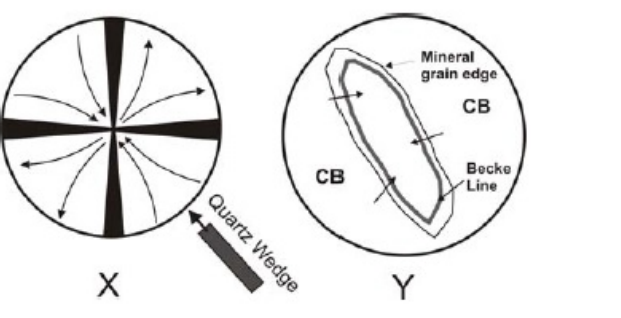
\includegraphics[width=0.4\textwidth]{figs/fig10.png}
    \caption{Image for questions 47}
    \label{fig:question47}
\end{figure}

\begin{multicols}{2}
\begin{enumerate}
\item Quartz, Stishovite  
\item Cordierite, Chlorite  
\item Apatite, Tourmaline  
\item Nosean, Halite  
\end{enumerate}
\end{multicols}

\item \textbf{(NAT)} From a recovered core of total length 200 cm, the RQD (Rock Quality Designation) is 

\begin{figure}[H]
    \centering
    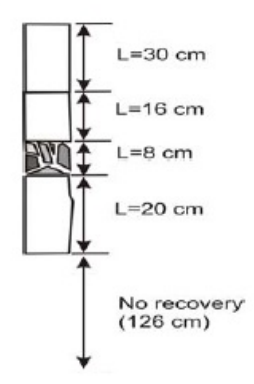
\includegraphics[width=0.2\textwidth]{figs/fig11.png}
    \caption{Image for questions 48}
    \label{fig:question48}
\end{figure}



\underline{\hspace{3cm}}\%.  
\vspace{0.3cm}

\item Interlimb angle and shape of a fold is best studied in a  
\begin{enumerate}
\item section parallel to the plunge of the fold axis  
\item section parallel to the axial plane of the fold  
\item section parallel to dip of bedding in the fold  
\item section whose pole is the fold axis  
\end{enumerate}

\item The thrust fault cross-section shows a hanging wall. Which combination is correct?  
\begin{figure}[H]
    \centering
    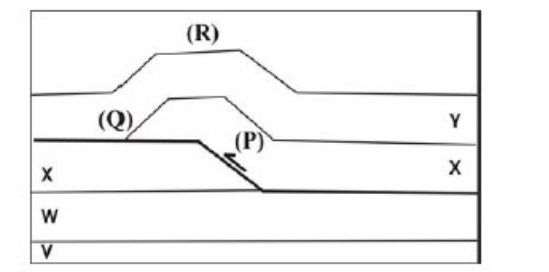
\includegraphics[width=0.4\textwidth]{figs/fig12.png}
    \caption{Image for questions 50}
    \label{fig:question28}
\end{figure}





\begin{enumerate}
\item Ramp (P), Flat (Q), Fault Bend Fold (R)  
\item Ramp (P), Flat (Q), Fault Propagation Fold (R)  
\item Flat (P), Ramp (Q), Fault Bend Fold (R)  
\item Flat (P), Ramp (Q), Fault Propagation Fold (R)  
\end{enumerate}

\item Euler Poles defined for plate motions on a spherical earth are  
\begin{enumerate}
\item parallel to associated transform faults  
\item perpendicular to associated transform faults  
\item not related to associated transform faults  
\item oblique to associated transform faults  
\end{enumerate}

\item Which one of the following sedimentary structures CANNOT be identified in vertical sections?  
\begin{multicols}{2}
\begin{enumerate}
\item Convolute lamination  
\item Gutter cast  
\item Dish structures  
\item Skip marks  
\end{enumerate}
\end{multicols}

\item A predominantly siliciclastic Mesozoic stratigraphic unit in mainland Kutch containing Trigonia and abundant plant fossils including Ptillophyllum is  
\begin{multicols}{2}
\begin{enumerate}
\item Baisakhi Formation  
\item Chari Formation  
\item Pachcham Formation  
\item Umia Formation  
\end{enumerate}
\end{multicols}

\item Match the texture in Group I with its corresponding description in Group II.

\begin{multicols}{2}
\textbf{Group I}  
\begin{flushleft}
P. Cumulus texture\\
Q. Exsolution texture\\
R. Caries texture\\
S. Cockade texture
\end{flushleft}

\columnbreak

\textbf{Group II}  
\begin{flushleft}
1. Triple point junction\\
2. Banding and crustification in open spaces\\
3. Protuberances of replacing mineral with replaced host\\
4. Spindles or lamellae of one mineral in another\\
5. Aggregates of minerals with non-penetrative mineral boundaries
\end{flushleft}
\end{multicols}

\begin{multicols}{2}
\begin{enumerate}
\item P--5; Q--4; R--3; S--2  
\item P--4; Q--5; R--3; S--1  
\item P--5; Q--4; R--2; S--3  
\item P--4; Q--3; R--2; S--5  
\end{enumerate}
\end{multicols}

\item Choose the CORRECT statement regarding coal.  
\begin{enumerate}
\item Sapropelic coal is a potential source rock of oil  
\item Vitrinite reflectance value (Ro \%) should be >1 for a lignite sample  
\item H/C content of the vitrinite maceral groups is more than that of liptinite maceral groups  
\item In Ranigunj field coal seams alternate with limestone beds  
\end{enumerate}

\end{enumerate}

\begin{enumerate}
\setcounter{enumi}{55}

\item Match the stratigraphic units in Group I with the economic deposits in Group II.

\begin{multicols}{2}
\textbf{Group I}  
\begin{flushleft}
P. Bailadila Group\\
Q. Nallamalai Group\\
R. Udaipur Group\\
S. Sausar Group
\end{flushleft}

\columnbreak

\textbf{Group II}  
\begin{flushleft}
1. Mn\\
2. Phosphorite\\
3. BIF\\
4. Pb-Zn\\
5. Pyrite
\end{flushleft}
\end{multicols}

\begin{multicols}{2}
\begin{enumerate}
\item P--3; Q--4; R--2; S--1  
\item P--4; Q--2; R--3; S--5  
\item P--2; Q--3; R--4; S--5  
\item P--3; Q--4; R--1; S--2  
\end{enumerate}
\end{multicols}

\item Match the igneous bodies in Group I with the cratons where they occur in Group II.

\begin{multicols}{2}
\textbf{Group I}  
\begin{flushleft}
P. Untala Granite\\
Q. Dalma Volcanics\\
R. Chamundi Granite\\
S. Bijli Rhyolite
\end{flushleft}

\columnbreak

\textbf{Group II}  
\begin{flushleft}
1. Singhbhum craton\\
2. Aravalli craton\\
3. Bastar craton\\
4. Dharwar craton\\
5. Bundelkhand craton
\end{flushleft}
\end{multicols}

\begin{multicols}{2}
\begin{enumerate}
\item P--2; Q--1; R--5; S--3  
\item P--2; Q--1; R--4; S--3  
\item P--3; Q--4; R--1; S--5  
\item P--1; Q--3; R--1; S--5  
\end{enumerate}
\end{multicols}

\item The reflectance spectrum of solar energy by hydrous molecules in plant leaves is best represented in the wavelength range of  
\begin{enumerate}
\item Near Infrared (0.7--1.3 μm)  
\item Short Infrared (1.3--3.0 μm)  
\item Mid Infrared (3--8 μm)  
\item Long Infrared (8--15 μm)  
\end{enumerate}


\item Match the type of mantled porphyroclasts in Group I with the corresponding figure in Group II.

\begin{figure}[H]
    \centering
    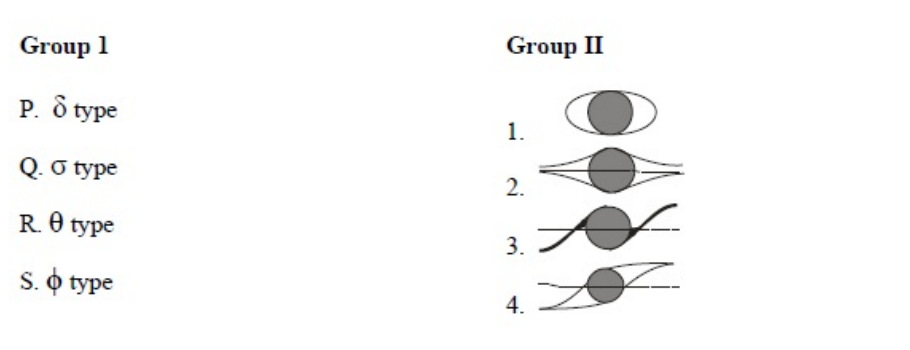
\includegraphics[width=0.6\textwidth]{figs/fig13.png}
    \caption{Image for questions 59}
    \label{fig:question59}
\end{figure}




\begin{multicols}{2}
\begin{enumerate}
\item P--3; Q--1; R--4; S--2  
\item P--3; Q--1; R--2; S--4  
\item P--1; Q--3; R--2; S--4  
\item P--2; Q--4; R--1; S--3  
\end{enumerate}
\end{multicols}


\item Choose the CORRECT symmetry operations that can create all possible two-dimensional planar point groups.  
\begin{enumerate}
\item translation, rotation, screw, glide  
\item translation, reflection, rotation, glide  
\item screw, reflection, rotation, glide  
\item translation, reflection, screw, glide  
\end{enumerate}

\item In the folded and faulted sequence of beds given in the map, the fault F--F (dipping 30° NE) is which type of fault?  

\begin{figure}[H]
    \centering
    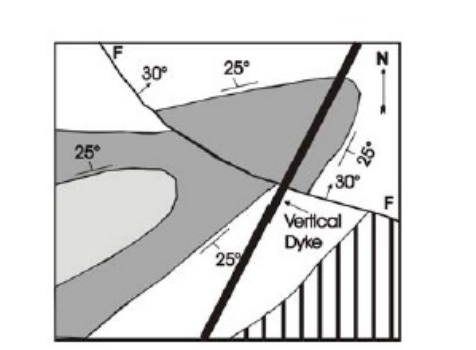
\includegraphics[width=0.4\textwidth]{figs/fig14.png}
    \caption{Image for questions 61}
    \label{fig:question61}
\end{figure}




\begin{multicols}{2}
\begin{enumerate}
\item sinistral strike-slip  
\item reverse  
\item normal  
\item dextral strike-slip  
\end{enumerate}
\end{multicols}

\item Which one of the following sets of isotopic ratios contains ONLY those that change with time?


\begin{enumerate}
\item \ensuremath{^{87}\text{Sr}/^{86}\text{Sr},\ \allowbreak ^{143}\text{Nd}/^{144}\text{Nd},\ \allowbreak ^{207}\text{Pb}/^{206}\text{Pb},\ \allowbreak ^{147}\text{Sm}/^{144}\text{Nd}}  
\item \ensuremath{^{88}\text{Sr}/^{86}\text{Sr},\ \allowbreak ^{145}\text{Nd}/^{144}\text{Nd},\ \allowbreak ^{238}\text{U}/^{204}\text{Pb},\ \allowbreak ^{207}\text{Pb}/^{204}\text{Pb}}  
\item \ensuremath{^{84}\text{Sr}/^{86}\text{Sr},\ \allowbreak ^{143}\text{Nd}/^{144}\text{Nd},\ \allowbreak ^{208}\text{Pb}/^{204}\text{Pb},\ \allowbreak ^{85}\text{Rb}/^{87}\text{Sr}}  
\item \ensuremath{^{145}\text{Nd}/^{144}\text{Nd},\ \allowbreak ^{86}\text{Sr}/^{84}\text{Sr},\ \allowbreak ^{147}\text{Sm}/^{144}\text{Nd},\ \allowbreak ^{208}\text{Pb}/^{86}\text{Sr}}  
\end{enumerate}


\item Sediments derived exclusively from the Deccan basalt are deposited on a high-energy beach and lithified under shallow burial conditions. The sedimentary rock formed would be a/an  
\begin{enumerate}
\item arkose  
\item greywacke  
\item lithic arenite  
\item quartz arenite  
\end{enumerate}

\item Choose the CORRECT mineral assemblages in mafic rocks that indicate eclogite facies metamorphism.  
\begin{enumerate}
\item $orthopyroxene + plagioclase + garnet  $
\item $glaucophane + omphacite + lawsonite + garnet $ 
\item $ugrandite garnet + omphacite + plagioclase  $
\item $pyralspite garnet + omphacite + kyanite  $
\end{enumerate}

\item The maximum velocity of the Indian Plate is observed in  
\begin{multicols}{4}
\begin{enumerate}
\item Maldives  
\item Bangalore  
\item Delhi  
\item Srinagar  
\end{enumerate}
\end{multicols}

\end{enumerate}
\newpage
\section*{Part B: Geophysics }
\vspace{0.7cm}
\begin{enumerate}
\setcounter{enumi}{65}

\item Which type of VES curve is obtained for a three-layered earth model consisting of wet shale (top layer), poorly water saturated sandstone (middle layer) and impermeable granite (bottom layer)?

\begin{multicols}{4}
\begin{enumerate}
\item K  
\item Q  
\item H  
\item A  
\end{enumerate}
\end{multicols}

\item In the estimation of magnetotelluric transfer function, the time-independent conservation of current at conductivity discontinuities will result in

\begin{multicols}{2}
\begin{enumerate}
\item phase rotation  
\item static-shift  
\item null tipper  
\item equal bi-modal apparent resistivity values  
\end{enumerate}
\end{multicols}

\item In any given signal, removal of all periods shorter than Nyquist period is achieved by

\begin{multicols}{2}
\begin{enumerate}
\item high-pass filtering  
\item band-pass filtering  
\item low-pass filtering  
\item band-reject filtering  
\end{enumerate}
\end{multicols}

\item The magnetic flux density \( \mathbf{B} \) and the magnetic vector potential \( \mathbf{A} \) are related by

\begin{multicols}{2}
\begin{enumerate}
\item \( \mathbf{B} = \nabla \cdot \mathbf{A} \)  
\item \( \mathbf{B} = \nabla \times \mathbf{A} \)  
\item \( \mathbf{A} = \nabla \mathbf{B} \)  
\item \( \mathbf{A} = \nabla \times \mathbf{B} \)  
\end{enumerate}
\end{multicols}

\item The frequency range (in Hz) that defines dead-band in magnetotelluric source signal is

\begin{multicols}{2}
\begin{enumerate}
\item 0.1--10  
\item 10--100  
\item 100--1000  
\item 1000--10000  
\end{enumerate}
\end{multicols}

\item \textbf{(NAT)} The maximum foldage obtained from a 48-channel common-depth-point (CDP) reflection survey with geophone and shot point spacing of 50 m and 100 m respectively is \underline{\hspace{2cm}}.

\item The deviation in the geographical locations of the magnetic poles from the geomagnetic poles of the Earth's magnetic field is due to

\begin{enumerate}
\item orientation of dipole axis  
\item external magnetic field  
\item non-dipole component  
\item ionospheric currents  
\end{enumerate}

\item The analytic signal for the function \( f(t) = \sin(\omega t) \) is

\begin{multicols}{4}
\begin{enumerate}
\item \( -\cos(\omega t) \)  
\item \( -\sin(\omega t) \)  
\item \( e^{i\omega t} \)  
\item \( -i e^{i\omega t} \)  
\end{enumerate}
\end{multicols}

\item \textbf{(NAT)} The minimum frequency at which a signal comprising of 30 Hz, 50 Hz and 70 Hz should be sampled to avoid aliasing is \underline{\hspace{2cm}} Hz.
\vspace{0.5cm}
\item Assertion (a): The Gutenberg-Richter frequency-magnitude relation of earthquakes globally suggests that subduction zones in general are characterized by lower b-values compared to mid-oceanic ridges.  
Reason (r): Earthquakes in subduction zones occur at deeper focal depths, whereas those along mid-oceanic ridges occur at shallow depths.

\begin{enumerate}
\item (a) is false but (r) is true  
\item Both (a) and (r) are true; and (r) is correct reason for (a)  
\item Both (a) and (r) are true; and (r) is not a reason for (a)  
\item Both (a) and (r) are false  
\end{enumerate}

\end{enumerate}

\begin{enumerate}
\setcounter{enumi}{75}

\item Deduce which one of the following statements is NOT correct from the given data on radioactive heat generation in Earth's layers:
\begin{table}[ht]
\centering
\begin{tabular}{|l|c|c|}
\hline
\textbf{Region} & \textbf{Mass ($\times 10^{21}$ kg)} & \textbf{Radioactive Heat Generation ($\times 10^8$ mWkg$^{-1}$)} \\
\hline
Upper continental crust & 8 & 96.40 \\
\hline
Lower continental crust & 8 & 40.00 \\
\hline
Oceanic crust & 7 & 18.60 \\
\hline
Mantle & 4080 & 0.26 \\
\hline
Core & 1880 & 0.00 \\
\hline
\end{tabular}
\end{table}


\begin{enumerate}
\item Core does not contain any radioactive isotope  
\item Lower continental crust is depleted in heat-producing elements compared to upper crust  
\item Mantle produces the highest radiogenic heat  
\item Upper continental crust produces the highest radiogenic heat  
\end{enumerate}

\item Which ONE of the following statements is CORRECT with regard to the application of reduction-to-pole (RTP) technique on magnetic anomaly maps?

\begin{enumerate}
\item RTP is efficient near the equator (below $\pm 20^\circ$ latitude)  
\item RTP assumes mainly induced magnetization  
\item RTP cannot be applied at higher latitudes (above $\pm 60^\circ$ latitude)  
\item RTP eliminates remnant magnetization sources  
\end{enumerate}

\item After migration, an anticline observed on an unmigrated seismic section becomes

\begin{multicols}{4}
\begin{enumerate}
\item broader  
\item tighter  
\item unaltered  
\item flat  
\end{enumerate}
\end{multicols}

\item A clean, thick, hydrocarbon-bearing sandstone bed can be identified through a combination of

\begin{enumerate}
\item low SP and high resistivity  
\item large SP and high resistivity  
\item low transit time and high resistivity  
\item large SP and low resistivity  
\end{enumerate}

\item \textbf{(NAT)} In a consolidated sandstone formation, the interval transit times of the formation, matrix, and fluid are 70 μs, 55 μs, and 190 μs respectively. The porosity of the formation is \underline{\hspace{2cm}}.

\item Which one of the following statements is NOT CORRECT?

\begin{enumerate}
\item A well-conditioned matrix has a condition number close to 1  
\item An ill-conditioned matrix has a large condition number  
\item The inverse of a well-conditioned matrix can be computed accurately  
\item A non-invertible matrix has a condition number close to 1  
\end{enumerate}

\item Match the type of inverse problem in Group I with its solution in Group II.

\begin{multicols}{2}
\textbf{Group I}  
\begin{flushleft}
P. Overdetermined\\
Q. Underdetermined\\
R. Mixed determined\\
S. Even determined
\end{flushleft}

\columnbreak

\textbf{Group II}  
\begin{flushleft}
1. \( m = [G^T G + k^2 I]^{-1} G^T d \)\\
2. \( m = (G^T G)^{-1} G^T d \)\\
3. \( m = G^T (G G^T)^{-1} d \)\\
4. \( m = (G G^T)^{-1} G^T d \)\\
5. \( m = G^{-1} d \)
\end{flushleft}
\end{multicols}

\begin{multicols}{2}
\begin{enumerate}
\item P--2; Q--4; R--1; S--5  
\item P--2; Q--3; R--1; S--5  
\item P--2; Q--1; R--3; S--4  
\item P--3; Q--5; R--2; S--1  
\end{enumerate}
\end{multicols}

\item In frequency domain IP, which frequency range (in Hz) is used to measure apparent resistivity at DC and AC limits?

\begin{multicols}{4}
\begin{enumerate}
\item 0.01--0.1  
\item 0.1--1  
\item 0.1--10  
\item 10--100  
\end{enumerate}
\end{multicols}

\item The expression for electrical potential \( V \) at a distance \( r \) from a subsurface point source of current in a homogeneous medium is

\begin{multicols}{4}
\begin{enumerate}
\item \( V = \frac{\rho I}{2\pi r} \)  
\item \( V = \frac{\rho I}{4\pi r} \)  
\item \( V = \frac{2\rho I}{\pi r} \)  
\item \( V = \frac{\rho r}{4\pi I} \)  
\end{enumerate}
\end{multicols}

\item The Bouguer anomaly obtained after applying all necessary corrections is due to

\begin{enumerate}
\item topographic undulations  
\item increase in crustal rock density with depth  
\item lateral density variations  
\item vertical density contrast across Moho  
\end{enumerate}


\end{enumerate}

\begin{enumerate}
\setcounter{enumi}{85}

\item In a 3-D seismic survey, the bin size for the maximum frequency ($f_{\text{max}} = 80$ Hz) at the target having a reflector dip of $15^\circ$ and interval velocity of $3600$ m/s is:

\textbf{(NAT)} \underline{\hspace{2cm}}

\vspace{0.5cm}

\item A spherical body with its centre located at a depth of 1040 m gives a symmetric residual gravity anomaly high with $\Delta g_{\text{max}} = 5.2$ mGal. If the same anomaly were to be obtained over a 2-D horizontal cylinder, the depth to the centre of the horizontal cylinder (in m) is:

\textbf{(NAT)} \underline{\hspace{2cm}}

\vspace{0.5cm}

\item Seismic velocities from a 3-component broadband station yield $V_p = 7.0$ km/s and $V_s = 3.87$ km/s for the lower crust. The Poisson's ratio of the lower crustal rocks is:

\begin{multicols}{4}
\begin{enumerate}
\item 0.24  
\item 0.26  
\item 0.28  
\item 0.30  
\end{enumerate}
\end{multicols}

\item Match the geometry of multiple reflections shown in Group I with their corresponding names in Group II.

\begin{figure}[H]
    \centering
    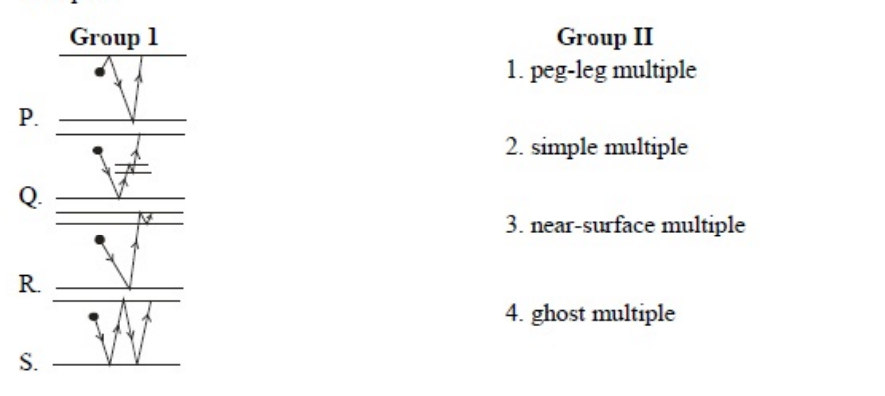
\includegraphics[width=0.6\textwidth]{figs/fig15.png}
    \caption{Image for questions 89}
    \label{fig:question89}
\end{figure}

\begin{multicols}{2}
\begin{enumerate}
\item P--1; Q--4; R--2; S--3  
\item P--4; Q--1; R--3; S--2  
\item P--2; Q--4; R--1; S--3  
\item P--3; Q--1; R--4; S--2  
\end{enumerate}
\end{multicols}

\item The Königsberger ratio $Q_u \ll 1$ is characteristic of:

\begin{multicols}{2}
\begin{enumerate}
\item Sandstone  
\item Continental shield rocks  
\item Oceanic basalt  
\item Continental volcanic rocks  
\end{enumerate}
\end{multicols}

\item In free-space, the integral form of Faraday's law is:

\begin{multicols}{4}
\begin{enumerate}
\item $\oint \vec{H} \cdot d\vec{l} = \iint \left( \frac{\partial \vec{E}}{\partial t} \right) d\vec{s}$  
\item $\oint \vec{E} \cdot d\vec{l} = - \iint \left( \frac{\partial \vec{B}}{\partial t} \right) d\vec{s}$  
\item $\iint \vec{E} \cdot d\vec{s} = 0$  
\item $\iint \vec{B} \cdot d\vec{s} = 0$  
\end{enumerate}
\end{multicols}

\item Four point charges $Q_1 = 40$ nC, $Q_2 = 50$ nC, $Q_3 = 20$ nC, $Q_4 = -60$ nC are enclosed by a Gaussian surface. The net flux crossing the surface is:

\textbf{(NAT)} \underline{\hspace{2cm}}

\vspace{0.5cm}

\item The highest frequency range (in Hz) of an inducing electromagnetic wave that can penetrate up to a depth of 178 m in a medium with resistivity $10\ \Omega\cdot$m is:

\begin{multicols}{4}
\begin{enumerate}
\item 1--10  
\item 15--25  
\item 70--100  
\item 800--1000  
\end{enumerate}
\end{multicols}

\item \textbf{(NAT)} For the given near-offset reflection geometry, the RMS velocity to the bottom of the second layer is:

\begin{figure}[H]
    \centering
    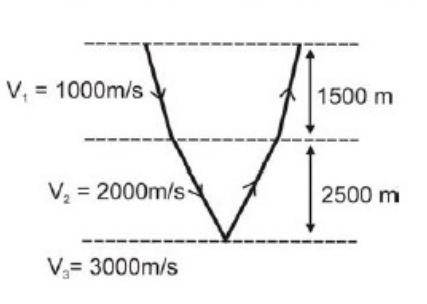
\includegraphics[width=0.4\textwidth]{figs/fig16.png}
    \caption{Image for questions 94}
    \label{fig:question94}
\end{figure}


\underline{\hspace{2cm}}

\end{enumerate}
\begin{enumerate}
\setcounter{enumi}{94}


\vspace{0.5cm}
\item In seismic exploration, the dynamite source is generally considered to be a wavelet of:

\begin{multicols}{2}
\begin{enumerate}
\item Zero phase  
\item Minimum phase  
\item Mixed phase  
\item Maximum phase  
\end{enumerate}
\end{multicols}
\end{enumerate}

\end{document}